%/*******************************************************************************
% * Copyright (c) 2009, medshare GmbH
% * All rights reserved. This program may not be distributed
% * or modified without prior written consent
% *
% * Contributors:
% *    T. Schaller - initial implementation
% *
% *******************************************************************************/
\documentclass[a4paper]{scrartcl}
\usepackage{german}
\usepackage[utf8]{inputenc}
\usepackage{makeidx}
\usepackage{wrapfig}
\makeindex

\usepackage[pdftex]{graphicx}
\DeclareGraphicsExtensions{.pdf,.jpg,.png}

\usepackage{floatflt}
\usepackage[]{hyperref}
\usepackage{color}
\title{Elexis - Afinion AS100 Connector}
\author{medshare GmbH}

\begin{document}

\maketitle
	\begin{center}
		
\includegraphics{elexis_logo}
	\end{center}
	\begin{center}
		
\includegraphics{axis-shield_logo}
	\end{center}
	\begin{center}
		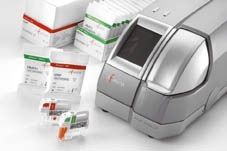
\includegraphics{afinion_device}
	\end{center}
	\begin{center}
		
\includegraphics{afinion_logo}
	\end{center}
\pagebreak

\section{Einf\"uhrung}
Dieses Plugin dient dazu, das Laborger\"at 'Afinion AS100 Analyzer'\footnote{Firma Axis-Shield} an Elexis anzubinden. Mit diesem Plugin k\"onnen die, vom Afinion gemessenen Laborparameter direkt in die Elexis-Datenbank eingelesen werden.

\subsection{Voraussetzungen}
Dieses Plugin ben\"otigt Elexis V1.4.1 oder h\"oher sowie einen Afinion AS100 Analyzer Ger\"at. Ausserdem wird ein PC mit mindestens einer freien seriellen Schnittstelle (Alternative: USB To RS-232 Adapter) und ein korrekt gerade verdrahtetes serielles Kabel (kein Nullmodemkabel) zur Verbindung des Afinion mit dem PC ben\"otigt.

\section{Installation und Konfiguration}
Installieren Sie auf dem, sich im Labor befindlichen PC das Plugin wie gewohnt. Verbinden Sie dann bei \textbf{ausgeschalteten} Ger\"aten den Afinion mit einem seriellen Port des Computers. 
\subsection{Daten\"ubertragungskonfiguration Afinion}
Die serielle Datenkommunikation ist im Afinion standardm\"assig aktiv. Das Ger\"at erfordert zwingend folgende Einstellungen:\\
Baudrate: 115200\\
Daten-Bits: 8\\
Parit\"at: Nein\\
Stop-Bits: 1
\subsection{Afinion Funktion Patienten-ID}
Die Funktion Patienten-ID ist auf dem Afinion Ger\"at standardm\"assig aktiviert. Mit dieser Funktion ist die Eingabe einer Patientenidentifikation bei jeder Probe auf dem Ger\"at zwingend. Wenn diese Funktion eingeschaltet, ist versucht Elexis den Patienten automatisch der Probe zuzuordnen. Wird die Funktion ausgeschaltet, muss in Elexis bei jeder Probe der Patient selektiert werden.\\
Weitere Informationen zur Funktion Patienten-ID finden Sie im Manual zum Afinion auf Seite 22.
\pagebreak
\subsection{Elexis Konfiguration}
Starten Sie Elexis und gehen Sie dort zu \textsc{Datei-Einstellungen-Datenaustausch- Afinion AS100 Analyzer} (S. Abb. \ref{fig:config}).
Hier stellen Sie den seriellen Port und die Schnittstellenparameter ein. Die Werte m\"ussen mit den Einstellungen auf dem Afinion Ger\"at \"ubereinstimmen (siehe oben). Wichtig: Nach dem \"Andern dieser Parameter m\"ussen Sie Elexis neu starten.\\
\\
\textbf{Weitere Konfigurationswerte:}\\
\textbf{Timeout (Sek):} Der Wert bestimmt, wie lange Elexis maximal auf Resultate warten soll, bevor die Verbindung getrennt wird.\\
\textbf{Im Hintergrund:} Damit beeinflussen Sie das Verhalten von Elexis. Bei eingeschalteter Option wird die \"Ubertragung im Hintergrund ausgef\"uhrt und sie k\"onnen weiter in Elexis arbeiten. Bei ausgeschalteter Option erscheint die Abb. \ref{fig:connected}\\
\textbf{Logging:} Diese Option verwenden Sie bitte nur auf Anweisung des Supports, ansonsten wird Ihr Computer mit unn\"otigen Daten gef\"ullt.\\
\begin{figure}[h]
    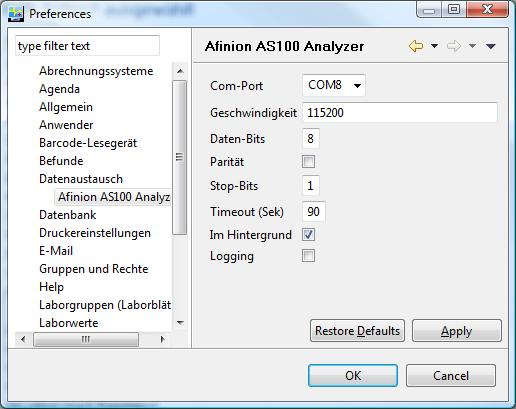
\includegraphics{config}
    \caption{Einstellungen Afinion AS100 Analyzer}
    \label{fig:config}
\end{figure}
\pagebreak
\section{Verwendung}
\begin{figure}[h]
    
\includegraphics{toolbarbutton}
    \caption{Afinion AS100 Analyzer Daten einlesen}
    \label{fig:toolbarbutton}
\end{figure}
Wenn das Plugin korrekt installiert ist, erscheint in der Labor-View automatisch ein neuer Toolbar Button 'Afinion AS100 Analyzer' (Abb. \ref{fig:toolbarbutton}).\\
\\
Ablauf:
\begin{enumerate}
\item Probenmessung mit dem Afinion durchf\"uhren
\item Messwert auf dem Afinion quittieren (allenfalls Patienten Nummer oder Namen eingeben)
\item Erst dann den Toolbar Button klicken um die Verbindung mit dem Ger\"at herzustellen.
\end{enumerate}
\begin{figure}[h]
    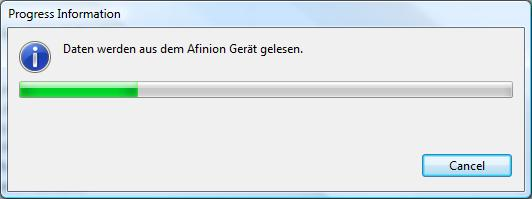
\includegraphics{connected}
    \caption{Verbindung zum Afinion ist aufgebaut}
    \label{fig:connected}
\end{figure}
Wenn Sie die Probe auf dem Afinion Ger\"at quittiert haben, k\"onnen Sie das Resultat mit einem Klick auf den Toolbar Button abholen. Wenn Elexis ein Resultat empf\"angt, wird versucht dieses einem Patienten zuzuordnen. In Abb. \ref{fig:messwert} ist ersichtlich, wie der Patient zugeordnet wird (Beispiel: Muster Franz sind die Angaben aus Elexis und MUSTER wurde auf dem Afinion eingegeben). Kann der Patient nicht automatisch zugewiesen werden folgt das Fenster mit der Patientenselektion.\\
\\
\\
\textbf{Wichtig:}\\
Es werden nur Werte an Elexis \"ubertragen, welche am aktuellen Tag gemessen wurden. \"Altere Messwerte m\"ussen Sie manuell in Elexis eingeben.
\begin{figure}[h]
    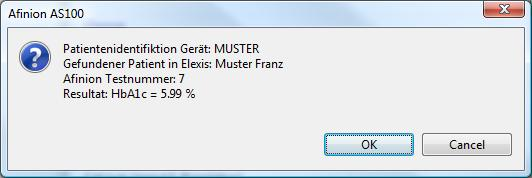
\includegraphics{messwert}
    \caption{Messwert vom Afinion eingetroffen}
    \label{fig:messwert}
\end{figure}

\subsection{Anweisungen zum Afinion}
Damit eine automatische Zuweisung des Patienten m\"oglich wird, muss auf dem Afinion der Patient der Messung zugeordnet werden (siehe auch 'Afinion Funktion Patienten-ID'). Auf dem Afinion kann die Patienten-ID numerisch oder als Text (Handy-Tastatur) eingegeben werden. Sie m\"ussen Sie zwingend eines der folgenden Eingabeformat einhalten (ohne Leerzeichen nach dem Komma!):\\
\begin{itemize}
\item \textbf{PatNummer}
\item \textbf{PatNummer,Namen}\\Tipp: Es kann auch nur der erste Buchstaben des Namens eingegeben werden
\item \textbf{Namen,Vornamen}\\Tipp: Namen und/oder Vornamen k\"onnen auch abgek\"urzt eingegeben werden
\end{itemize}

\section{Fehlerbehandlung}
Wenn das Ger\"at nicht reagiert k\"onnen die Verbindung mit Cancel gem\"ass Abb. \ref{fig:connected} abbrechen. Ansonsten bleibt die Verbindung bis zum Ablauf des konfigurierten Timeouts bestehen.\\
\section{Plattformen}
Dieses Plugin wurde unter Windows XP und Vista getestet. Beachten Sie bitte, dass unter Linux die seriellen Ports nicht COM1 usw., sondern /dev/ttyS0 usw. heissen.

\section{Kabelspezifikation}
Es wird ein normales serielles Kabel ben\"otigt (kein Nullmodemkabel!). Das Kabel muss vom 9-poligen Stecker (m\"annlich) auf den 9-poligen Stecker (weiblich) 1:1 verdrahtet sein. Folgende Pins werden verwendet: 2 (Receive), 3 (Transmit), 5 (Signal GND).\\

\end{document}
